\begin{problem}
Copie el programa~\ref{code:elliptic1D.m} y modifique lo siguiente:

\begin{itemize}
      \item

            Cambie el orden de precisión a $4$.

      \item

            Asigne el número de celdas a $10$.

      \item

            Mantenga las condiciones de frontera de tipo Robin.

      \item

            Cambie la función de fuerza a $f\left(x\right)=1+x$.

      \item

            Ejecute el programa con todos los cambios que ha realizado.

      \item

            Verifique que la gráfica es apropiada (títulos, valores de los ejes, etc.).
\end{itemize}
\end{problem}

\begin{solution}
      Se está resolviendo la ecuación de Poisson con el
      problema de valor de frontera Robin
      \begin{equation*}
            \left\{
            \begin{aligned}
                  \diff[2]{u}{x}
                   & =1+x,
                  \text{ para }x\in\left[0,1\right].     \\
                  0
                   & = u\left(0\right)-\diff{u}{x}[x=0]. \\
                  2e
                   & =u\left(1\right)+\diff{u}{x}[x=1].  \\
            \end{aligned}
            \right.
      \end{equation*}

      Integramos dos veces y obtenemos la solución general.
      \begin{align*}
            \iint
            \diff[2]{u}{x}
            \dl x
            \dl x           & =
            \iint
            \left(1+x\right)
            \dl x
            \dl x.              \\
            \int
            \diff{u}{x}
            \dl x           & =
            \int
            \left(x+\frac{x^{2}}{2}+C_{1}\right)
            \dl x.              \\
            u\left(x\right) & =
            \frac{x^{2}}{2}+\frac{x^{3}}{6}+C_{1}x+C_{2}.
      \end{align*}
      Ahora, apliquemos las condiciones de frontera Robin.
      \begin{equation}
            \left\{
            \begin{aligned}
                  0
                   & =
                  u\left(0\right)-
                  \diff{u}{x}[x=0]=
                  C_{2}-C_{1}. \\
                  2e
                   & =
                  u\left(1\right)+
                  \diff{u}{x}[x=1]=
                  \frac{13}{6}+2C_{1}+C_{2}.
            \end{aligned}
            \right.
      \end{equation}
      Así el sistema tiene como solución
      $C_{1}=C_{2}=\frac{2e}{3}-\frac{13}{18}$.
      Así, la solución exacta
      de~\eqref{eq:poisson1drobindconditions} es
      \begin{math}
            u\left(x\right)=
            \frac{x^{2}}{2}+\frac{x^{3}}{6}+
            \left(x+1\right)\left(\frac{2e}{3}-\frac{13}{18}\right)
      \end{math}.
      % You may write claims, lemmas, propositions, etc. inside your solution.
      % \begin{lemma}\label{lem}
      %     Some auxiliary result.
      % \end{lemma}
      % \begin{proof}
      %     The proof of \cref{lem}, where we use the following formula:
      %     \[
      %         \infty = \infty + 1.
      %         \qedhere % For placing the Q.E.D. symbol in the right place.
      %     \]
      % \end{proof}
      % \begin{fact}[This statement requires no proof]
      %     \proofless % To change the hollow box marking the end of a theorem-type environment into a solid one.
      %     Some statement.
      % \end{fact}
      % ... and the rest steps...
      \noQED
\end{solution}

\begin{figure}[ht!]
      \centering
      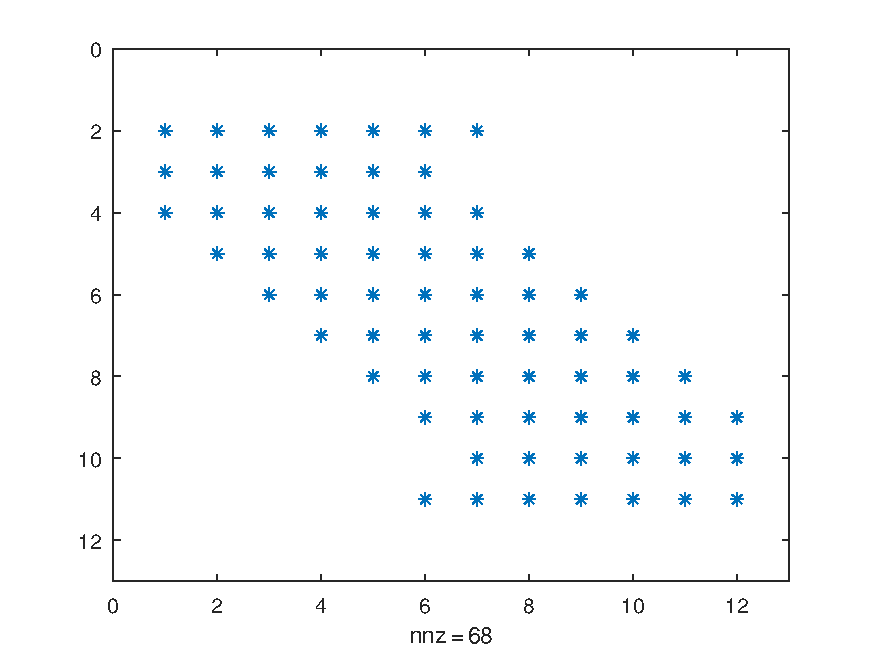
\includegraphics[width=.39\paperwidth]{elliptic1D_Aznaran_sparsebefore.pdf}
      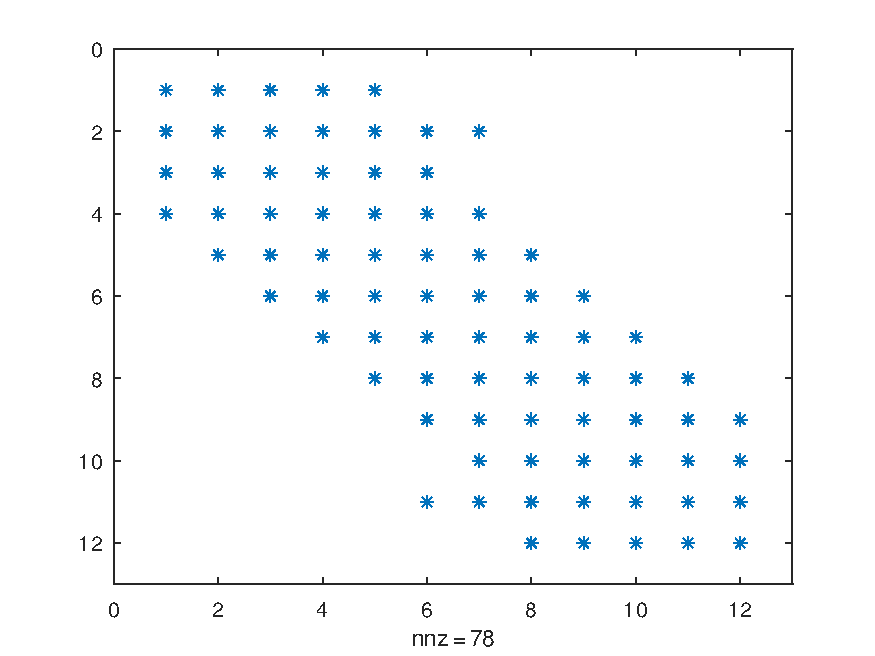
\includegraphics[width=.39\paperwidth]{elliptic1D_Aznaran_sparseafter.pdf}
      % \caption{Izquierda: Representación dispersa de $L$ hasta la línea 21.
      %     La primera fila y última fila son vectores nulos.
      %     Derecha: Representación dispersa de $L$ hasta la línea 29.
      %     La matriz $L\in\mathbb{R}^{15\times 15}$.}
\end{figure}

\begin{figure}[ht!]
      \centering
      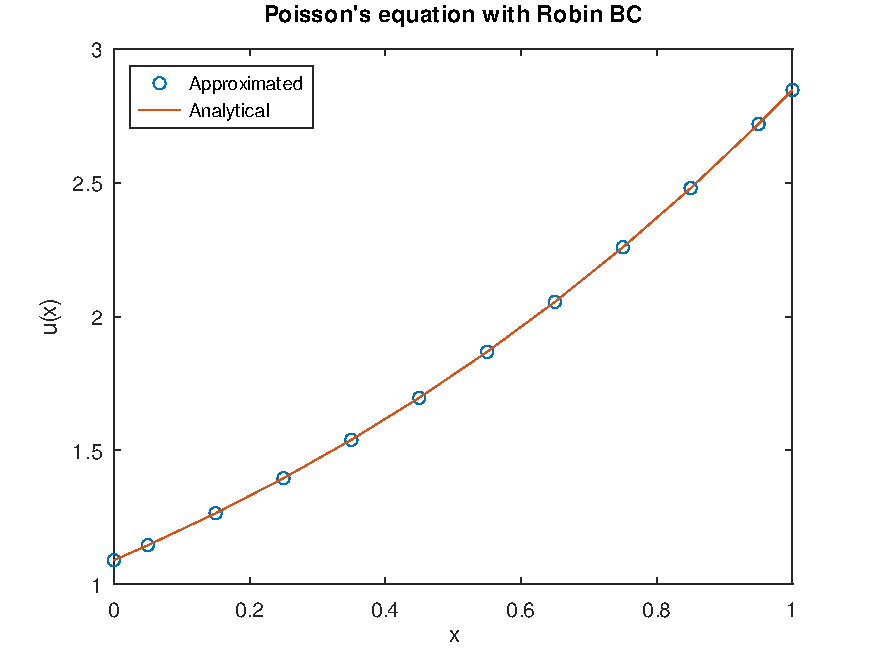
\includegraphics[width=.6\paperwidth]{elliptic1D_Aznaran.pdf}
      % \caption{Solución al problema usando \mintinline{octave}|k=6| y \mintinline{octave}|m=2k+1=13|.}
\end{figure}

% En la línea $4$, la función
% \href{https://docs.octave.org/latest/Cursor-Motion.html#index-clc}{\mintinline{octave}|clc|}
% limpia la pantalla del terminal y mueve el cursor a la esquina superior izquierda.

% En la línea $5$, la función
% \href{https://docs.octave.org/latest/Manipulation-of-Plot-Windows.html#index-close-3}{\mintinline{octave}|close all|}
% cierra todas las ventanas de las figuras con manejadores visibles.
% \url{https://docs.octave.org/v9.3.0/Creating-Sparse-Matrices.html}
% \url{https://docs.octave.org/v9.3.0/Information.html}
% \url{https://www.mathworks.com/matlabcentral/fileexchange/44354-curvilinear-2d-grid-poisson}